%%%%%%%%%%%%%%%%%%%%%%%%%%%%%%%%%%%%%%
% LaTeX poster template
% Created by Nathaniel Johnston
% August 2009
% http://www.nathanieljohnston.com/2009/08/latex-poster-template/
%%%%%%%%%%%%%%%%%%%%%%%%%%%%%%%%%%%%%%

\documentclass[final]{beamer}
\usepackage[orientation=portrait, size=arch, scale=1.3]{beamerposter}
\usepackage{graphicx}
\usepackage[noabbrev,capitalize]{cleveref}
\usepackage{wrapfig}
\usepackage[sharp]{easylist}
\usepackage{tikz}

\setlength{\paperwidth}{36in}
\setlength{\paperheight}{48in}
\setlength{\topmargin}{0cm}%

\newlength{\sepwid}
\newlength{\onecolwid}
\newlength{\twocolwid}
%% For three columns
\setlength{\sepwid}{0.024\paperwidth}
\setlength{\onecolwid}{0.47\paperwidth}  % (1-(3+1)*0.024)/3 = 0.30133333
\setlength{\twocolwid}{2\onecolwid}

\usetheme{confposter}
\usepackage{exscale}

\usecaptiontemplate{
\small
\structure{\insertcaptionname~\insertcaptionnumber:}
\insertcaption}
%-----------------------------------------------------------
% Name and authors of poster/paper/research
%-----------------------------------------------------------

\title{A Browser-based MEI Editor}
\author{ 
    \vspace{0.3\baselineskip} 
    \normalsize
    Andrew Horwitz (ahwitz@gmail.com), Andrew Hankinson (andrew.hankinson@mail.mcgill.ca), Ichiro Fujinaga (ich@music.mcgill.ca)
}
\institute{
    \vspace{0.2\baselineskip} 
    \normalsize Distributed Digital Music Archives and Libraries Lab, CIRMMT, Schulich School of Music, McGill University
}

\newcommand{\blockSpace}{\vskip 0.75ex}
\newcommand*{\xml}[1]{\small{\texttt{<#1>}}\normalsize}
\newcommand*{\att}[1]{\small{\texttt{@#1}}\normalsize}

%-----------------------------------------------------------
% Start the poster itself
%-----------------------------------------------------------
\begin{document}
% ensure 5cm of space at the top
\setlength{\voffset}{1 in}%

% ----------
% The Poster
% ----------
\begin{frame}[fragile,t]
  \vspace{4cm}
  \begin{minipage}[t][.8\textheight]{\textwidth}
    \begin{columns}
    \begin{column}{0.00\textwidth}
    \end{column}

    \begin{column}{0.95\textwidth}
        \vspace{-4.8cm}
        \begin{block}{}
        \vspace{-4cm}
        \begin{columns}
        \begin{column}{0.47\textwidth}
            \vspace{1cm}
            \begin{block}{Motivation}
The SIMSSA project aims to create searchable representations of musical sources. We have started by identifying neumes in early chant manuscripts via optical music recognition; because the MEI output of the recognition process is not perfectly accurate, we have developed an interface that:

                \vspace{0.5\baselineskip}
                \begin{easylist}[itemize]
                \ListProperties(Margin1=0cm)
# Allows users to edit MEI files manually
# Can open multiple files simultaneously and can save them from the browser to a user's computer
# Links files with their representations in other browser-based MEI editing applications and synchronizes changes
                \end{easylist}
                \vspace{0.5\baselineskip}

We are using this application to edit manuscripts from the St. Gallen monastery, and are developing a prototype Verovio editor.
            \end{block}
            \blockSpace{}
        \end{column}

        \begin{column}{0.00cm}
        \end{column}

        \begin{column}{0.47\textwidth}
            \begin{block}{The JS MEI Editor (meix.js)}

                \begin{center}
                    \vspace{-0.75\baselineskip}
                    \small{https://github.com/DDMAL/meix.js}
                    \normalsize
                    \vspace{0.25\baselineskip}
                \end{center}
                \begin{easylist}[itemize]
                \ListProperties(Margin1=0cm, Margin2=3cm)
        # JavaScript library using the ACE Text Editor$^1$:
        ## ACE features: XML syntax highlighting, find and replace, and code folding, among others
        ## Tabbed view for opening multiple MEI files simultaneously
        # Provides XML validation with custom MEI schemas:
        ## Emscripten$^2$-compiled version of xmllint and WebWorker interface allows validation in the browser
        ## Custom Node.js server that interfaces with command-line xmllint allows online validation
        # Has a well-documented plugin structure for integration with other applications
                \end{easylist}
            \end{block}
            \blockSpace{}
        \end{column}
        \end{columns}
        \end{block}

        \vspace{2cm}
        \begin{block}{}
        \vspace{-5.5cm}
        \begin{columns}
        \begin{column}{0.47\textwidth}
            \begin{block}{}
            \hspace{-1cm}
                \centering
                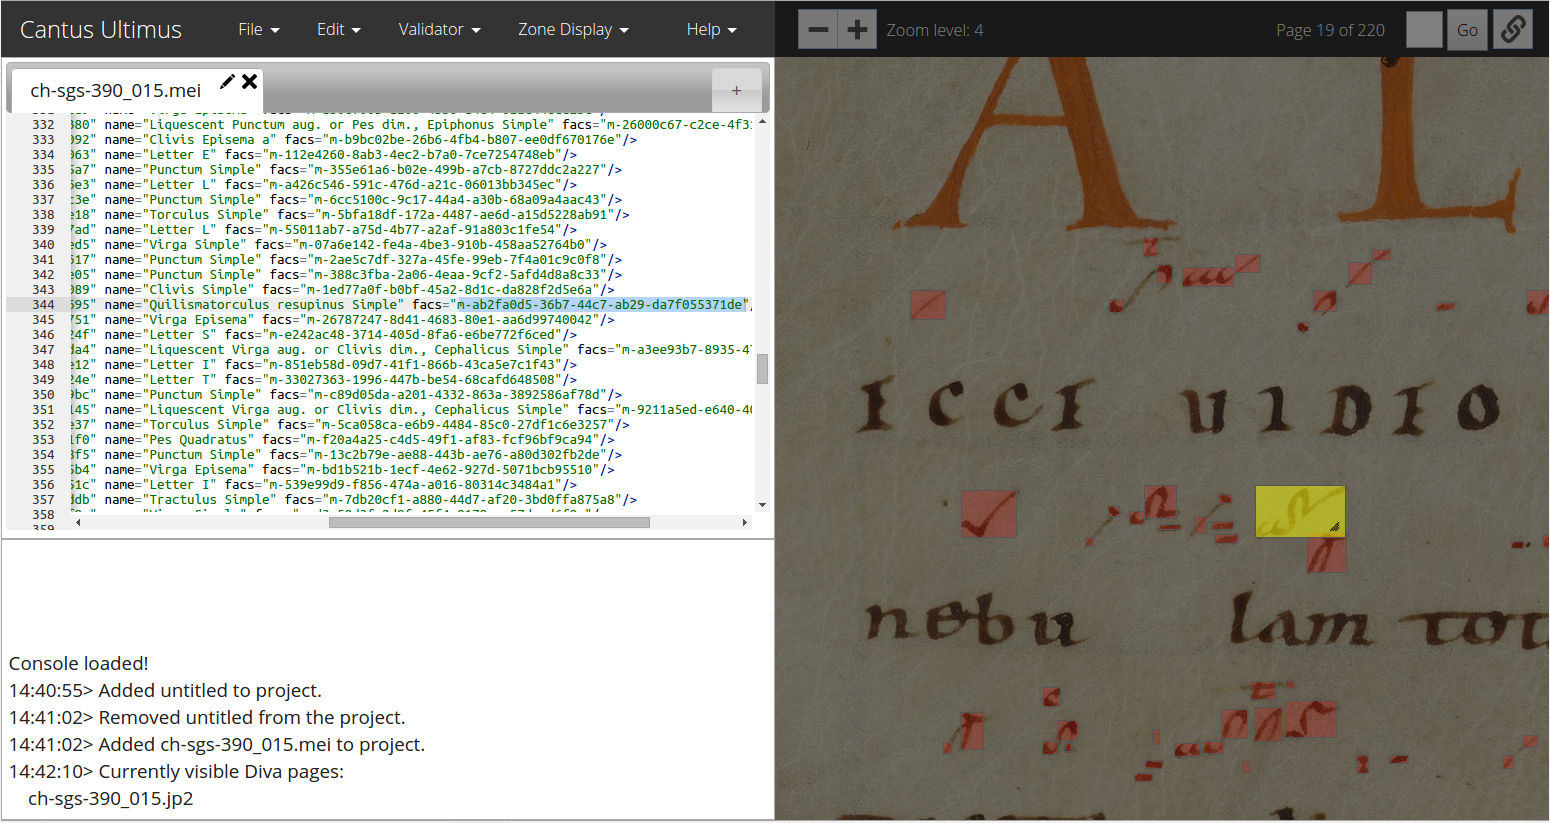
\includegraphics[scale=0.75]{mei_editor_diva}
            \end{block}
        \blockSpace{}
        \end{column}

        \begin{column}{0.00cm}
        \end{column}

        \begin{column}{0.47\textwidth}
            \begin{block}{}
                \centering
                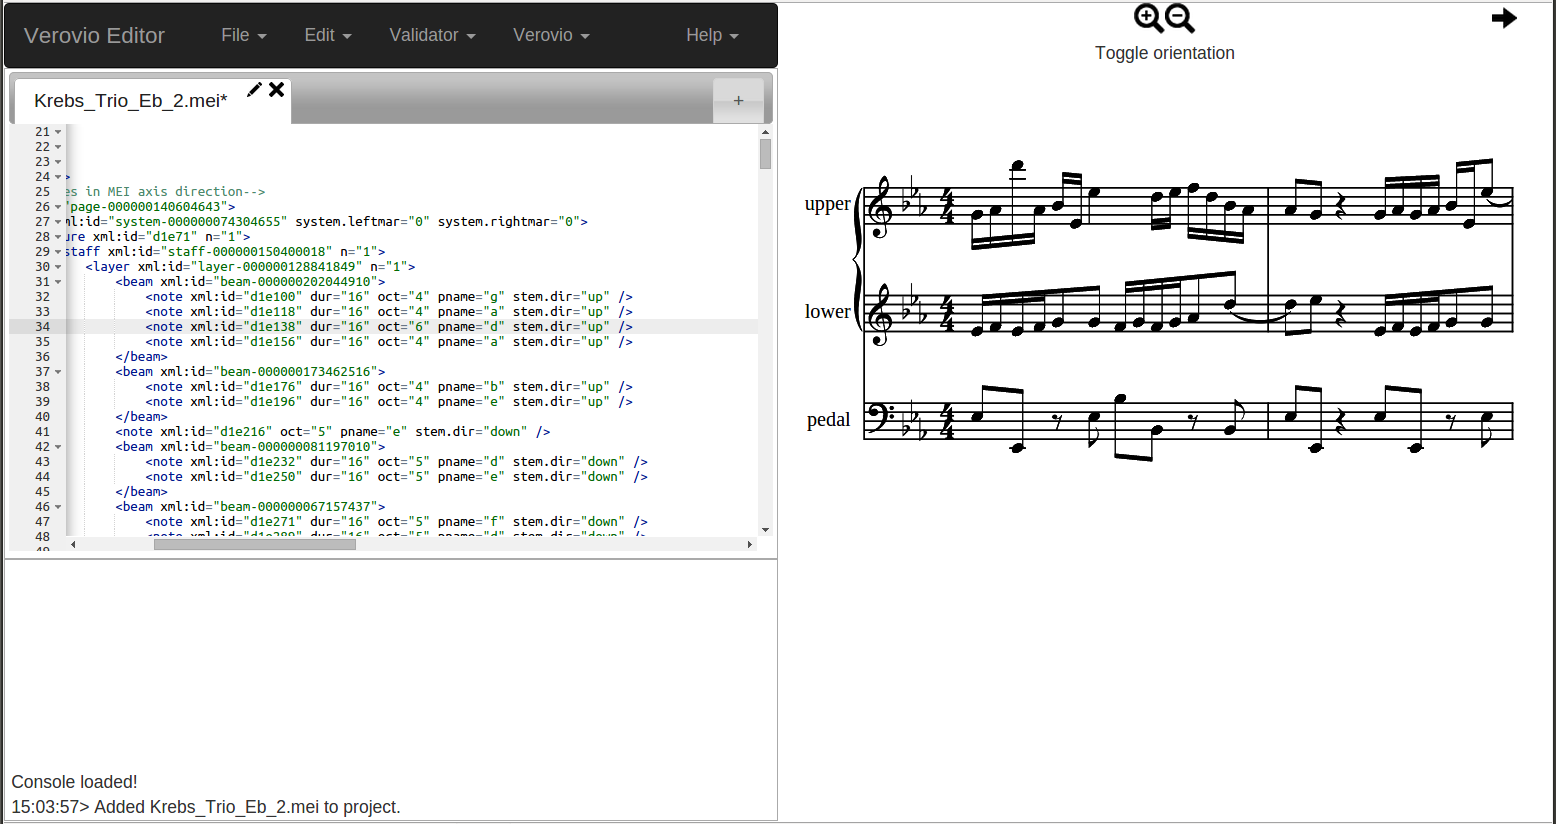
\includegraphics[scale=0.75]{mei_editor_verovio}
            \end{block}
            \blockSpace{}
        \end{column}
        \end{columns}
        \end{block}

        \vspace{2cm}
        \begin{block}{}
        \vspace{-3cm}
        \begin{columns}
        \begin{column}{0.47\textwidth}
            \vspace{-.5cm}
            \begin{block}{St. Gallen}
            \begin{center}
                \vspace{-0.75\baselineskip}
                \small{http://dev-cantus.simssa.ca/editor/}
                \normalsize
                \vspace{0.25\baselineskip}
            \end{center}
    
            meix.js synchronizes with a Diva.js$^3$ document viewer pane for editing MEI representations of music manuscripts.
                
                \vspace{0.5\baselineskip}
                \begin{easylist}[itemize]
                \ListProperties(Margin1=0cm)
    # Editing the MEI \xml{zone} elements changes the positioning and size of the highlighted areas
    # Dragging/resizing the highlighted areas changes the \att{ulx}/\att{uly}/\att{lrx}/\att{lry} values of the \xml{zone} elements
    # Users can manually create new zones, which are then automatically inserted in the proper location in the MEI
    # Hundreds of pages in a manuscript are linked to corresponding MEI files and automatically loaded
    # Hovering over a highlight displays all attributes associated with the musical object linked to the \xml{zone}
                \end{easylist}

                \vspace{4cm}
                \centering
                \includegraphics[scale=1.9]{highlight_atts}

            \end{block}
        \blockSpace{}
        \end{column}

        \begin{column}{0.00cm}
        \end{column}

        \begin{column}{0.47\textwidth}
            \begin{block}{Verovio}
                \begin{center}
                    \vspace{-0.75\baselineskip}
                    \small{http://dev.simssa.ca/veditor/}
                    \normalsize
                    \vspace{0.25\baselineskip}
                \end{center}

    meix.js synchronizes with a Verovio$^4$-generated score with drag-and-drop editing functionality.

                \vspace{0.5\baselineskip}

                \begin{easylist}[itemize]
                \ListProperties(Margin1=0cm)
    # Based on editor prototype at http://rism-ch.github.io/verovio/mei-editor.xhtml
    # Dragging and dropping an element in Verovio re-renders the score and updates the MEI
    # Manually editing the MEI regenerates the score
    # Score automatically paginates by dividing MEI into systems dependent on page width  
                \end{easylist}

            \end{block}
            \blockSpace{}

            \vspace{1.5cm}

            \begin{block}{References}
            \small
            [1] http://ace.c9.io/

            [2] http://mozakai.blogspot.ca/2012/03/howto-port-cc-library-to-javascript.html

            [3] https://ddmal.github.io/diva.js/

            [4] http://rism-ch.github.io/verovio/index.xhtml
            \end{block}   


            \vfill

            \begin{block}{Acknowledgements}
            \small
            This research was supported by the Social Sciences and Humanities Research Council of Canada.
            \end{block}

            \begin{block}{}
                \centering
                \raisebox{0.7cm}{
\includegraphics[scale=0.12]{images/McGill_logo}}
                \hspace{1.2cm} 
                \raisebox{0.1cm}{
\includegraphics[scale=0.5]{images/Schulich_logo}}
                \hspace{0.6cm} 
                
\includegraphics[scale=0.16]{images/CIRMMT_logo}

                
\includegraphics[scale=1.4]{images/SSHRC_logo}
                \vspace{0.8cm}

                
\includegraphics[scale=0.3]{images/ddmal_logo_large}
                \hspace{1.3cm}
                
\includegraphics[scale=0.9]{images/SIMSSA_logo}
            \end{block}
        \end{column}
        \end{columns}
        \end{block}

    \end{column}

\begin{column}{0.00\textwidth}
\end{column}
\end{columns}
\end{minipage}
\end{frame}
\end{document}
